% -*- coding: utf-8 -*-
%-------------------------designed by zcf--------------
\documentclass[UTF8,a4paper,10pt]{ctexart}
\usepackage[left=3.17cm, right=3.17cm, top=2.74cm, bottom=2.74cm]{geometry}
\usepackage{amsmath}
\usepackage{graphicx,subfig}
\usepackage{float}
\usepackage{cite}
\usepackage{caption}
\usepackage{enumerate}
\usepackage{booktabs}
\usepackage{multirow}
\usepackage{array}
\newcommand{\tabincell}[2]{\begin{tabular}{@{}#1@{}}#2\end{tabular}}
%-------------------------字体设置--------------
\usepackage{ctex}
\setCJKmainfont[ItalicFont=Noto Sans CJK SC Bold, BoldFont=Noto Serif CJK SC Black]{Noto Serif CJK SC}
\newcommand{\yihao}{\fontsize{26pt}{36pt}\selectfont}
\newcommand{\erhao}{\fontsize{22pt}{28pt}\selectfont}
\newcommand{\xiaoer}{\fontsize{18pt}{18pt}\selectfont}
\newcommand{\sanhao}{\fontsize{16pt}{24pt}\selectfont}
\newcommand{\xiaosan}{\fontsize{15pt}{22pt}\selectfont}
\newcommand{\sihao}{\fontsize{14pt}{21pt}\selectfont}
\newcommand{\banxiaosi}{\fontsize{13pt}{19.5pt}\selectfont}
\newcommand{\xiaosi}{\fontsize{12pt}{18pt}\selectfont}
\newcommand{\dawuhao}{\fontsize{11pt}{11pt}\selectfont}
\newcommand{\wuhao}{\fontsize{10.5pt}{15.75pt}\selectfont}
%-------------------------章节名----------------
\usepackage{ctexcap}
\CTEXsetup[name={,、},number={ \chinese{section}}]{section}
\CTEXsetup[name={（,）},number={\chinese{subsection}}]{subsection}
\CTEXsetup[name={,.},number={\arabic{subsubsection}}]{subsubsection}
%-------------------------页眉页脚--------------
\usepackage{fancyhdr}
\pagestyle{fancy}
\lhead{\kaishu \leftmark}
\rhead{\kaishu 并行程序设计实验报告}
\lfoot{}
\cfoot{\thepage}
\rfoot{}
\renewcommand{\headrulewidth}{0.1pt}
\renewcommand{\footrulewidth}{0pt}
\newcommand{\HRule}{\rule{\linewidth}{0.5mm}}
\newcommand{\HRulegrossa}{\rule{\linewidth}{1.2mm}}
%-----------------------伪代码------------------
\usepackage{algorithm}
\usepackage{algorithmicx}
\usepackage{algpseudocode}
\floatname{algorithm}{Algorithm}
\renewcommand{\algorithmicrequire}{\textbf{Input:}}
\renewcommand{\algorithmicensure}{\textbf{Output:}}
\usepackage{lipsum}
\makeatletter
\newenvironment{breakablealgorithm}
  {% \begin{breakablealgorithm}
  \begin{center}
     \refstepcounter{algorithm}% New algorithm
     \hrule height.8pt depth0pt \kern2pt%
     \renewcommand{\caption}[2][\relax]{%
      {\raggedright\textbf{\ALG@name~\thealgorithm} ##2\par}%
      \ifx\relax##1\relax
         \addcontentsline{loa}{algorithm}{\protect\numberline{\thealgorithm}##2}%
      \else
         \addcontentsline{loa}{algorithm}{\protect\numberline{\thealgorithm}##1}%
      \fi
      \kern2pt\hrule\kern2pt
     }
  }{% \end{breakablealgorithm}
     \kern2pt\hrule\relax%
  \end{center}
  }
\makeatother
%------------------------代码-------------------
\usepackage{xcolor}
\usepackage{listings}
\lstset{
breaklines,
basicstyle=\small,
escapeinside=``,
keywordstyle=\color{ blue!70} \bfseries,
commentstyle=\color{red!50!green!50!blue!50},
stringstyle=\ttfamily,
extendedchars=false,
linewidth=\textwidth,
numbers=left,
numberstyle=\tiny \color{blue!50},
frame=trbl
rulesepcolor= \color{ red!20!green!20!blue!20}
}
%------------超链接----------
\usepackage[colorlinks,linkcolor=black,anchorcolor=blue]{hyperref}
%------------------------水印-------------------
\usepackage{tikz}
\usepackage{xcolor}
\usepackage{eso-pic}

\newcommand{\watermark}[3]{\AddToShipoutPictureBG{
\parbox[b][\paperheight]{\paperwidth}{
\vfill%
\centering%
\tikz[remember picture, overlay]%
  \node [rotate = #1, scale = #2] at (current page.center)%
    {\textcolor{gray!80!cyan!30!magenta!30}{#3}};
\vfill}}}



%———————————————————————————————————————————正文———————————————————————————————————————————————
%----------------------------------------------
\begin{document}
\begin{titlepage}
    \begin{center}
    
\includegraphics[width=0.8\textwidth]{NKU.png}\\[1cm]
    \textsc{\Huge \kaishu{\textbf{南\ \ \ \ \ \ 开\ \ \ \ \ \ 大\ \ \ \ \ \ 学}} }\\[0.9cm]
    \textsc{\huge \kaishu{\textbf{计\ \ 算\ \ 机\ \ 学\ \ 院}}}\\[0.5cm]
    \textsc{\Large \textbf{并行程序设计期末实验报告}}\\[0.8cm]
    \HRule \\[0.9cm]
    { \LARGE \bfseries SIMD编程}\\[0.4cm]
    \HRule \\[2.0cm]
    \centering
    \textsc{\LARGE \kaishu{刘华彬}}\\[0.5cm]
    \textsc{\LARGE \kaishu{年级\ :\ 大二}}\\[0.5cm]
    \textsc{\LARGE \kaishu{专业\ :\ 计算机科学与技术}}\\[0.5cm]
    \textsc{\LARGE \kaishu{指导教师\ :\ 崔立骁}}\\[0.5cm]
    \vfill
    {\Large \today}
    \end{center}
\end{titlepage}
%-------------摘------要--------------
\newpage
\thispagestyle{empty}
\renewcommand{\abstractname}{\kaishu \sihao \textbf{摘要}}
    \begin{abstract}
        \noindent

本次SIMD编程实践，基于ARM NEON SIMD指令集，设计并实现了4路并行的MD5哈希加速方案。核心思路是利用MD5中FF、GG、HH、II四个轮函数仅涉及简单位运算且无分支的特性，同时计算4条口令的哈希值。在此基础上，本文设计了AoS到SoA的数据布局转置方案以实现高效的SIMD数据加载，并采用栈缓冲区策略减少堆内存分配开销。实验结果表明，在华为鲲鹏920 ARM服务器上，-O1编译选项下Hash时间从3.00s降至1.11s（加速比2.70x），-O2下从2.95s降至1.05s（加速比2.81x）。进一步结合perf性能剖析与汇编分析，本文详细讨论了编译优化选项对SIMD程序性能的影响机制，以及在-O0下SIMD程序性能退化的根本原因。\textbf{项目源代码：} \url{https://github.com/BLH549/NKU_Parallel}
\end{abstract}
%----------------------------------------------------------------
\tableofcontents
%----------------------------------------------------------------
\newpage
\watermark{60}{10}{NKU}
\setcounter{page}{1}

%======================= 1. 问题描述 =======================
\section{问题描述}

\subsection{口令猜测与MD5哈希}

口令猜测是口令安全研究中的基础问题。攻击者通过生成大量候选口令并计算其哈希值，与泄露的哈希值进行比对来破解用户口令。本次作业基于PCFG（Probabilistic Context-Free Grammar）模型，按照概率降序生成候选口令，并使用MD5算法计算每条口令的哈希值。

在整个口令猜测流水线中，MD5哈希计算是主要的时间开销之一。在串行实现中，框架逐条调用MD5Hash函数对口令进行哈希。由于PCFG生成的口令数量可达千万级别，且各条口令的哈希计算之间不存在数据依赖，因此MD5哈希是天然的并行化目标。本SIMD编程实验聚焦于利用ARM NEON向量指令集，实现对多条口令MD5哈希的并行计算。

\subsection{SIMD编程实验子问题}

本实验的具体任务为：在ARM服务器（华为鲲鹏920）上，基于NEON Intrinsics实现MD5哈希算法的SIMD并行化，使得单次函数调用能同时生成多条口令的哈希值。要求在保证哈希结果正确的前提下，获得可观的加速比，并结合perf等性能剖析工具对程序性能进行深入分析。

%======================= 2. 串行MD5算法分析 =======================
\section{串行MD5算法分析}

\subsection{MD5算法流程}

MD5算法对输入消息的处理分为以下步骤：

\begin{enumerate}
  \item \textbf{消息填充}：将消息填充至长度模512bit余448bit，并附加64bit的原始消息长度字段，使最终长度为512bit的整数倍。此部分在框架的\lstinline{StringProcess}函数中完成。
  \item \textbf{分组处理}：将填充后的消息按512bit（64字节）划分为若干块（block），每个块再划分为16个32bit的字（记为$x[0..15]$）。
  \item \textbf{缓冲区更新}：维护128bit的缓冲区，由4个32bit寄存器$A,B,C,D$组成。对每个512bit块，以该块的字$x[0..15]$为输入，依次执行4轮（Round 1-4）、每轮16步的运算，更新$A,B,C,D$的值。全部块处理完毕后，缓冲区中的值即为MD5哈希结果。
\end{enumerate}

\subsection{关键函数与并行机会}

每一轮运算中，每一步执行的操作由以下四个宏函数之一定义：

\begin{lstlisting}[title=串行MD5轮函数宏定义,frame=trbl,language={C++}]
#define F(x, y, z) (((x) & (y)) | ((~x) & (z)))
#define G(x, y, z) (((x) & (z)) | ((y) & (~z)))
#define H(x, y, z) ((x) ^ (y) ^ (z))
#define I(x, y, z) ((y) ^ ((x) | (~z)))

#define FF(a, b, c, d, x, s, ac) { \
  (a) += F((b), (c), (d)) + (x) + ac; \
  (a) = ROTATELEFT((a), (s)); \
  (a) += (b); \
}
// GG, HH, II 结构相同，仅替换F为G, H, I
\end{lstlisting}

分析上述函数可以发现以下有利于SIMD并行化的特征：

\begin{enumerate}
  \item \textbf{无分支判断}：FF/GG/HH/II四个宏均不包含条件分支（if-else），控制流完全确定。
  \item \textbf{仅涉及简单运算}：操作仅为按位与/或/非/异或、模$2^{32}$加法、循环左移。这些运算在NEON指令集中均有直接的对应指令。
  \item \textbf{数据高度对齐}：所有操作数均为32bit无符号整数，每次操作的数据宽度相同，天然适合4路32bit SIMD（NEON的\lstinline{uint32x4_t}）。
  \item \textbf{口令间无数据依赖}：不同口令的哈希计算完全独立，不存在跨口令的数据依赖，可以在SIMD寄存器中分别处理。
\end{enumerate}

并行化的基本思路是：将4条不同口令的同一运算步骤打包到NEON的128bit向量寄存器中，使用向量指令替换标量指令，一次完成4条口令的同步计算。形式上，设串行版本中寄存器$(a,b,c,d)$分别维护一条口令的中间状态，则SIMD版本中$(\mathbf{A},\mathbf{B},\mathbf{C},\mathbf{D})$各自为包含4条口令对应状态值的向量寄存器。每个标量运算提升为对应的向量运算，例如标量FF中的按位与操作，在SIMD版本中变为\lstinline{vandq_u32}。

%======================= 3. SIMD算法设计与实现 =======================
\section{SIMD算法设计与实现}

\subsection{4路NEON并行化策略}

本方案选择4路并行（对应NEON的128bit寄存器宽度），每次同时处理4条口令的MD5哈希计算。串行MD5中的宏函数FF/GG/HH/II被替换为对应的NEON向量宏VFF/VGG/VHH/VII。以VFF为例：

\begin{lstlisting}[title=SIMD向量化轮函数宏定义,frame=trbl,language={C++}]
#define VFN(x, y, z) vorrq_u32(vandq_u32((x),(y)), vandq_u32(vmvnq_u32((x)),(z)))
#define VROTATEL(val, n) vorrq_u32(vshlq_n_u32((val),(n)), \
                                   vshrq_n_u32((val),(32-(n))))

#define VFF(a, b, c, d, x, s, ac) { \
    (a) = vaddq_u32((a), VFN((b), (c), (d))); \
    (a) = vaddq_u32((a), (x)); \
    (a) = vaddq_u32((a), vdupq_n_u32(static_cast<uint32_t>(ac))); \
    (a) = VROTATEL((a), (s)); \
    (a) = vaddq_u32((a), (b)); \
}
\end{lstlisting}

其中\lstinline{VFN}是标量宏$F(x,y,z) = (x \land y) \lor (\lnot x \land z)$的向量化翻译：\lstinline{vandq_u32}对应按位与，\lstinline{vmvnq_u32}对应按位取反，\lstinline{vorrq_u32}对应按位或。\lstinline{VROTATEL}通过左移和右移的组合实现循环左移。GG/HH/II的向量化方式类似，仅替换核心布尔函数。以上宏定义直接展开到调用处，避免了函数调用开销（在-O0下尤为重要）。

\subsection{AoS到SoA的数据布局转置}

原始代码框架以AoS（Array of Structures）方式组织数据：每条口令的消息块中，16个32bit字按顺序存储（$p_0[x_0..x_{15}]$, $p_1[x_0..x_{15}]$, ...）。但SIMD需要SoA（Structure of Arrays）布局：4条口令的第$k$个字应被打包在同一个向量寄存器中（$x_k = \{p_0[k], p_1[k], p_2[k], p_3[k]\}$）。

为此，本方案在每轮运算前进行AoS→SoA的4×4矩阵转置。使用NEON的\lstinline{vzipq_u32}指令完成，该指令对两个向量进行交织（interleave）操作，通过两轮zip即可实现转置：

\begin{lstlisting}[title=AoS到SoA的4×4矩阵转置,frame=trbl,language={C++}]
// 从4条口令中加载4个连续32bit字 (AoS布局)
uint32x4_t m0 = vld1q_u32((const uint32_t*)&padded[0][off]);
uint32x4_t m1 = vld1q_u32((const uint32_t*)&padded[1][off]);
uint32x4_t m2 = vld1q_u32((const uint32_t*)&padded[2][off]);
uint32x4_t m3 = vld1q_u32((const uint32_t*)&padded[3][off]);

// 两轮zip实现转置: AoS -> SoA
uint32x4x2_t t0 = vzipq_u32(m0, m2);
uint32x4x2_t t1 = vzipq_u32(m1, m3);
uint32x4x2_t u0 = vzipq_u32(t0.val[0], t1.val[0]);
uint32x4x2_t u1 = vzipq_u32(t0.val[1], t1.val[1]);

// 转置结果: x[k*4+0..3]中，每个向量包含4条口令的同一个32bit字
x[k * 4 + 0] = u0.val[0]; // 4条口令的第(k*4+0)个字
x[k * 4 + 1] = u0.val[1];
x[k * 4 + 2] = u1.val[0];
x[k * 4 + 3] = u1.val[1];
\end{lstlisting}

该转置过程在16个字上仅需8条NEON指令（4条vld + 4条vzip），相比逐字节重组方案大大降低了指令开销。转置完成后，$x[0]..x[15]$即为SoA布局的16个向量，可以直接用于后续的VFF/VGG/VHH/VII运算。

\subsection{栈缓冲区与内存优化}

串行MD5的\lstinline{StringProcess}函数每次调用都会通过\lstinline{new[]}在堆上分配填充后的消息缓冲区。在大规模口令猜测场景中（每100万条口令触发一次批量哈希），频繁的堆分配与释放会带来显著的开销。此外，常见口令长度（$<$100字符）对应的填充消息长度不超过128字节。

本方案采用栈优先策略：在栈上预分配128字节对齐的缓冲区，当填充长度$\leq 128$时直接使用栈缓冲区，仅在超长口令时回退到堆分配。由于绝大多数口令长度在合理范围内，该优化几乎消除了每批次的内存分配开销，同时提升了数据在L1缓存中的局部性。

\begin{lstlisting}[title=栈优先缓冲区策略,frame=trbl,language={C++}]
alignas(16) Byte padded_buf[4][128]; // 4条口令的栈缓冲区, 16字节对齐
Byte* padded[4];
bool on_heap[4] = {false};

for (int i = 0; i < batch_count; i++) {
    int plen = ((input_len + 72) / 64) * 64;
    if (plen <= 128) {
        padded[i] = padded_buf[i];        // 栈: 零分配开销
    } else {
        padded[i] = new Byte[plen];       // 堆: 仅超长口令回退
        on_heap[i] = true;
    }
    // 消息填充 ...
}
\end{lstlisting}

\subsection{算法伪代码}

\begin{breakablealgorithm}
  \caption{NEON SIMD批量MD5哈希}
  \begin{algorithmic}[1]
      \Require 口令数组 $inputs[0..count-1]$, 口令数量 $count$
      \Ensure 哈希结果数组 $states[0..count-1][0..3]$
      \State $BATCH\_SIZE \gets 4$
      \For {$batch\_start \gets 0$ \textbf{to} $count-1$ \textbf{step} $BATCH\_SIZE$}
          \State $batch\_count \gets$ 当前批次的剩余口令数（$\leq 4$）
          \For {$i \gets 0$ \textbf{to} $batch\_count-1$}
              \State 对$inputs[batch\_start+i]$进行消息填充，优先使用栈缓冲区
          \EndFor
          \State 补齐不足4条的批次（指针别名至最后一条，只读语义）
          \State $\mathbf{A},\mathbf{B},\mathbf{C},\mathbf{D} \gets$ 初始IV向量（4条口令各一份）
          \For {每个512bit消息块}
              \State 4$\times$4矩阵转置: AoS $\to$ SoA，生成$x[0..15]$向量
              \State Round 1: 16次 \textbf{VFF} 运算（使用$x[0..15]$的指定项）
              \State Round 2: 16次 \textbf{VGG} 运算
              \State Round 3: 16次 \textbf{VHH} 运算
              \State Round 4: 16次 \textbf{VII} 运算
              \State $\mathbf{A},\mathbf{B},\mathbf{C},\mathbf{D} \mathrel{+}= \mathbf{a},\mathbf{b},\mathbf{c},\mathbf{d}$
          \EndFor
          \State 从向量寄存器提取4条口令的最终哈希值（小端转大端）
          \State 清理堆缓冲区（如有）
      \EndFor
  \end{algorithmic}
\end{breakablealgorithm}

\subsection{复杂性分析}

设口令总数为$N$，每条口令的消息块数为$B$。串行MD5Hash的时间复杂度为$O(N \cdot B)$，每条口令需独立执行$64B$次标量运算（4轮$\times$16步）。

SIMD版本将4条口令合并处理，本质是将常数因子缩小为原来的$1/4$。但引入以下额外开销：
\begin{itemize}
  \item AoS→SoA转置：每消息块需8条NEON指令（$O(B)$量级，每条口令摊销2条）
  \item 补齐不足4条的批次：通过指针别名实现，开销可忽略
  \item 标量常量复制：通过\lstinline{vdupq_n_u32}实现，每条指令可并行广播
\end{itemize}

理论加速比受限于SIMD宽度（4路）和额外开销的比例。实际加速比取决于额外开销能否被编译器优化（内联、寄存器分配等）所抵消，这正是不同编译选项下表现差异巨大的原因。

%======================= 4. 实验与结果分析 =======================
\section{实验与结果分析}

\subsection{实验环境}

\begin{table}[!htbp]
  \centering
  \begin{tabular}{ll}
  \toprule
  项目 & 配置 \\
  \midrule
  CPU & 华为鲲鹏920（ARMv8-A架构，支持NEON） \\
  操作系统 & openEuler（Linux） \\
  编译器 & g++ (GCC)，支持ARM NEON Intrinsics \\
  编译选项 & -O0（无优化）、-O1、-O2 \\
  NEON头文件 & \texttt{<arm\_neon.h>} \\
  性能分析工具 & perf（Linux性能剖析器） \\
  猜测生成数量 & 10,000,000条口令 \\
  \bottomrule
  \end{tabular}
  \caption{实验环境配置}
  \label{tab:env}
\end{table}

\subsection{正确性验证}

首先使用8组标准测试向量验证SIMD版本的MD5输出正确性。测试口令及预期哈希值如表\ref{tab:correctness}所示。SIMD版本（4路并行）对所有测试口令均产生与串行版本完全一致的哈希结果，验证了向量化实现的正确性。

\begin{table}[!htbp]
  \centering
  \begin{tabular}{cl}
  \toprule
  口令 & 预期MD5哈希值 \\
  \midrule
  123456 & e10adc3949ba59abbe56e057f20f883e \\
  password & 5f4dcc3b5aa765d61d8327deb882cf99 \\
  12345678 & 25d55ad283aa400af464c76d713c07ad \\
  qwerty & d8578edf8458ce06fbc5bb76a58c5ca4 \\
  123456789 & 25f9e794323b453885f5181f1b624d0b \\
  12345 & 827ccb0eea8a706c4c34a16891f84e7b \\
  1234 & 81dc9bdb52d04dc20036dbd8313ed055 \\
  111111 & 96e79218965eb72c92a549dd5a330112 \\
  \bottomrule
  \end{tabular}
  \caption{MD5正确性测试向量}
  \label{tab:correctness}
\end{table}

\subsection{不同编译选项下的加速比}

\subsubsection{完整程序Hash时间对比}

表\ref{tab:full-hash}和图\ref{fig:speedup}给出了串行baseline与最终SIMD优化版本在三种编译优化级别下的Hash时间及加速比（Hash time指程序执行MD5哈希计算的总时间，不包含训练和猜测生成时间）。

\begin{table}[!htbp]
  \centering
  \begin{tabular}{cccccc}
  \toprule
  \multirow{2}{*}{编译选项} & \multicolumn{2}{c}{串行baseline} & \multicolumn{2}{c}{SIMD（最终版）} & \multirow{2}{*}{加速比} \\
  \cmidrule(lr){2-3} \cmidrule(lr){4-5}
  & Hash time(s) & 单次($\mu$s) & Hash time(s) & 单次($\mu$s) & \\
  \midrule
  -O0 & 9.31 & 0.931 & 12.33 & 1.233 & 0.76$\times$ \\
  -O1 & 3.00 & 0.300 & 1.11 & 0.111 & 2.70$\times$ \\
  -O2 & 2.95 & 0.295 & 1.05 & 0.105 & 2.81$\times$ \\
  \bottomrule
  \end{tabular}
  \caption{完整程序Hash时间对比（10M条口令）}
  \label{tab:full-hash}
\end{table}

\begin{figure}[H]
    \centering
    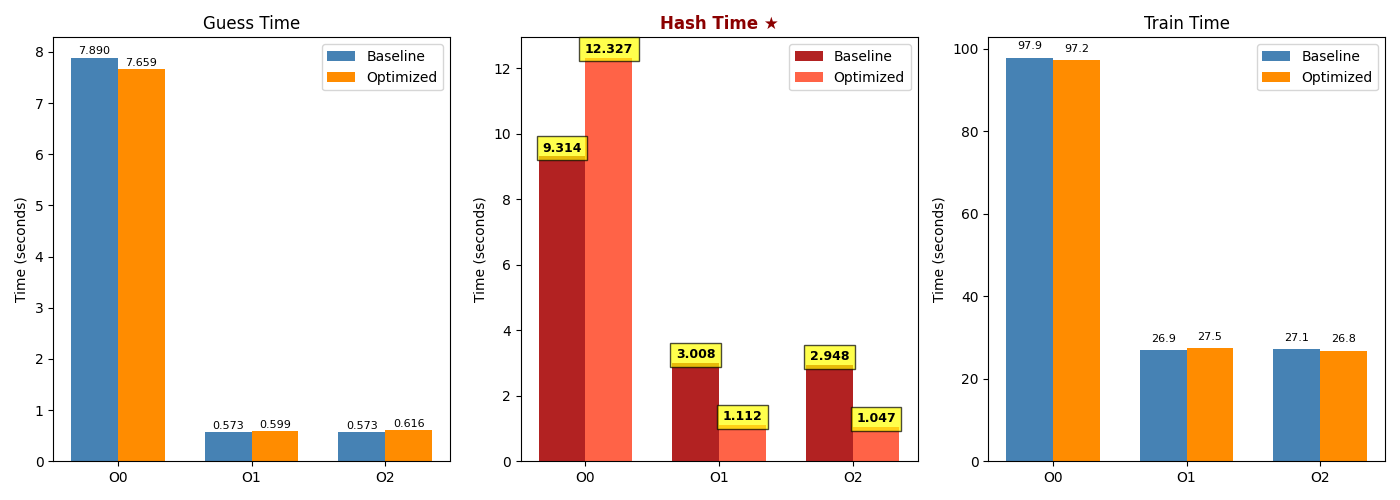
\includegraphics[scale=0.4]{Guess_TimeCost.png}
    \caption{不同编译选项下时间对比（完整程序）}
    \label{fig:speedup}
\end{figure}

\subsubsection{纯MD5测试}

为进一步排除PCFG猜测生成、训练阶段等干扰因素，使用独立的MD5性能测试程序（\texttt{test\_md5\_serial}和\texttt{test\_md5\_simd}），对8条固定口令重复计算800,000次，结果如表\ref{tab:micro}所示。

\begin{table}[!htbp]
  \centering
  \begin{tabular}{ccccc}
  \toprule
  编译选项 & 串行单次($\mu$s) & SIMD单次($\mu$s) & 加速比 \\
  \midrule
  -O0 & 0.941 & 1.436 & 0.66$\times$ \\
  -O1 & 0.295 & 0.201 & 1.47$\times$ \\
  -O2 & 0.302 & 0.191 & 1.58$\times$ \\
  \bottomrule
  \end{tabular}
  \caption{纯MD5微基准测试结果（800,000次调用）}
  \label{tab:micro}
\end{table}

\subsubsection{加速比数据分析}

\noindent\textbf{（1）完整程序加速比高于微基准的现象}

一个值得注意的现象是：完整程序的SIMD加速比（O1: 2.70$\times$, O2: 2.81$\times$）显著高于纯MD5微基准的加速比（O1: 1.47$\times$, O2: 1.58$\times$）。原因分析如下：

\begin{itemize}
  \item \textbf{规模化摊销}：完整程序每次批量处理100万条口令，SIMD版本中的转置开销、对齐开销被大规模数据摊销；而微基准每次仅处理8条口令的100,000次迭代循环，循环开销和调用开销占比较大。
  \item \textbf{栈缓冲区效益放大}：在大批量场景下，栈缓冲区策略消除了1M次堆分配，内存访问模式更规整，L1缓存命中率更高。
\end{itemize}

\noindent\textbf{（2）-O0下性能退化的根本原因}

在 -O0 优化选项下，SIMD 版本不仅未能实现加速，反而出现了明显的性能回退。结合后文的汇编分析可知，这是由于 -O0 采用了“计算即访存”的保守策略。本文将在第 \ref{sec:explore} 节通过底层汇编特征对此现象进行分析。
\subsection{perf性能剖析}

\subsubsection{完整程序perf对比（-O1）}

使用perf stat对串行和SIMD版本的完整程序进行性能剖析，结果如表\ref{tab:perf-full}所示。

\begin{table}[!htbp]
  \centering
  \begin{tabular}{lcc}
  \toprule
  指标 & 串行（baseline -O1） & SIMD（最终版 -O1） \\
  \midrule
  总执行时间（s） & 38.73 & 36.41 \\
  CPU周期数（B） & 98.30 & 91.83 \\
  指令数（B） & 60.43 & 47.80 \\
  IPC & 0.61 & 0.52 \\
  L1数据缓存加载（B） & 21.73 & 18.64 \\
  L1数据缓存未命中率 & 4.29\% & 5.05\% \\
  LLC加载（B） & 1.70 & 1.68 \\
  LLC未命中率 & 15.01\% & 16.80\% \\
  \bottomrule
  \end{tabular}
  \caption{完整程序perf stat对比（-O1）}
  \label{tab:perf-full}
\end{table}

从perf数据分析可得：

\begin{enumerate}
  \item \textbf{指令数减少21\%}：从60.43B降至47.80B，验证了SIMD减少了实际执行的运算指令数。这与4路并行的理论预期（减少约75\%的运算指令）存在差距，原因在于引入了转置、补齐等额外指令。
  \item \textbf{IPC从0.61降至0.52}：SIMD版本的IPC反而更低。这是由于NEON向量指令的延迟高于简单标量指令，且转置操作中\lstinline{vzipq_u32}涉及跨通道的数据重排，需要额外的执行周期。
  \item \textbf{缓存行为接近}：两个版本的L1和LLC缓存表现相似，说明栈缓冲区优化有效避免了额外访存。L1未命中率略有增加（4.29\% $\to$ 5.05\%），主要由4条口令数据同时在L1中竞争所致。
\end{enumerate}

\subsubsection{纯MD5的perf对比（-O1）}

为排除PCFG训练和猜测生成阶段的干扰，对纯MD5微基准测试程序进行perf剖析。表\ref{tab:perf-md5}给出了串行与SIMD版本的完整对比。

\begin{table}[!htbp]
  \centering
  \begin{tabular}{lcc}
  \toprule
  指标 & 串行（-O1） & SIMD（-O1） \\
  \midrule
  总执行时间（ms） & 239 & 164 \\
  CPU周期数（M） & 615 & 421 \\
  指令数（M） & 1,354 & 837 \\
  IPC & 2.20 & 1.99 \\
  L1数据缓存加载（M） & 317 & 247 \\
  L1数据缓存未命中率 & 0.004\% & 0.005\% \\
  LLC未命中率 & 54.3\% & 59.0\% \\
  \bottomrule
  \end{tabular}
  \caption{纯MD5微基准perf stat对比（-O1）}
  \label{tab:perf-md5}
\end{table}

从对比数据可得以下结论：

\begin{enumerate}
  \item \textbf{指令数减少38\%}（1,354M $\to$ 837M）：验证了SIMD有效减少了核心运算指令数。与理论预期的75\%指令减少存在差距，原因在于转置指令（vzip）和常量广播（vdup）引入了额外开销。
  \item \textbf{IPC轻微下降}（2.20 $\to$ 1.99）：串行版本的标量指令可充分利用乱序执行和流水线，而NEON向量指令（尤其是vzip跨通道操作）具有更高的执行延迟。但1.99的IPC仍然处于高位，说明NEON流水线利用率良好。
  \item \textbf{L1缓存行为极优}：双版本L1未命中率均低于0.01\%，说明纯MD5计算的工作集完全适配L1缓存。这归功于数据规模小（8条口令的填充消息）且访问模式规整。
  \item \textbf{LLC未命中率看似较高但绝对值极小}：LLC加载仅约12,000次，未命中约7,000次，绝对数量可忽略不计，属于程序启动阶段的冷启动未命中。

\end{enumerate}


%======================= 5. 探索与优化历程 =======================
\section{进阶探索与优化历程}
\label{sec:explore}

\subsection{编译优化选项对加速比的影响机制}

图\ref{fig:speedup}展示了-O0/-O1/-O2三种编译选项下加速比的巨大差异：-O0下为负加速（0.76$\times$），-O1下跳升至2.70$\times$，-O2下进一步小幅提升至2.81$\times$。其机制分析如下：

\noindent\textbf{-O0（无优化）：} 尽管 NEON Intrinsic 通常会被正确展开为底层 NEON 汇编指令，但由于 -O0 完全禁用了寄存器分配优化，编译器采取了极其保守的执行策略（每条语句的中间结果必须立刻写回内存）。这导致 MD5 计算中频繁产生的 128-bit 向量变量被不断溢出（spill）并重载（reload）到庞大的栈帧中，引发了严重的内存读写开销与缓存抖动（关于此负优化现象的详细汇编级证明见本章第三节），从而彻底抵消了向量化带来的并行收益。

\noindent\textbf{-O1（基本优化）：} 编译器开启了关键的寄存器分配优化与基本的指令调度。活跃的 SIMD 数据得以常驻于 NEON 的向量寄存器堆中，彻底消除了 -O0 阶段灾难性的栈访存瓶颈。此时，vadd 等向量指令能够真正高效地直接操作寄存器，SIMD 的算力得以释放，这是加速比产生质变飞跃的核心原因。

\noindent\textbf{-O2（更强优化）：} 在-O1基础上进一步加强指令调度、循环优化等。由于MD5算法本身具有严格的指令级依赖链（每一步依赖前一步的$a$值），-O2的额外优化空间有限，这也是-O2相较-O1提升不大（2.70$\times$ $\to$ 2.81$\times$）的原因。

\subsection{从初版到最终版的优化路径}

本实验经历了多轮迭代优化。初版SIMD实现直接在原始框架上替换FF/GG/HH/II为NEON版本（使用内联函数而非宏），并在每次调用中通过\lstinline{new[]}分配填充消息缓冲区。表\ref{tab:evolution}记录了两个主要版本的性能对比。

\begin{table}[!htbp]
  \centering
  \begin{tabular}{cccccc}
  \toprule
  \multirow{2}{*}{版本} & \multicolumn{3}{c}{Hash time（s）} & \multicolumn{2}{c}{加速比} \\
  \cmidrule(lr){2-4} \cmidrule(lr){5-6}
  & -O0 & -O1 & -O2 & -O1 & -O2 \\
  \midrule
  串行baseline & 9.31 & 3.00 & 2.95 & --- & --- \\
  初版SIMD & 19.27 & 1.82 & 1.71 & 1.65$\times$ & 1.72$\times$ \\
  最终版SIMD & 12.33 & 1.11 & 1.05 & 2.70$\times$ & 2.81$\times$ \\
  \bottomrule
  \end{tabular}
  \caption{版本迭代性能对比}
  \label{tab:evolution}
\end{table}

最终版相比初版的主要改进如下：

\begin{enumerate}
  \item \textbf{宏替换函数}：初版使用内联函数封装NEON操作，在-O0下产生大量真实的函数调用。最终版改为类函数宏（\lstinline{#define VFF ...}），保证在任何编译选项下都直接展开为内联的NEON Intrinsic调用序列，消除了函数调用边界。
  \item \textbf{AoS→SoA转置}：初版在数据加载时使用逐元素排列的方式组织SIMD数据，需要大量的\lstinline{vsetq_lane}操作。最终版改为矩阵转置方案（\lstinline{vzipq_u32}）。
  \item \textbf{栈缓冲区替代堆分配}：初版每次填充都进行\lstinline{new[]}/\lstinline{delete[]}。最终版使用栈缓冲区（128字节对齐），在10M口令规模下避免了约2,500次堆分配/释放，同时保持数据在L1缓存的热度。
  \item \textbf{StringProcess传参与计算简化}：原\lstinline{StringProcess}函数按值接受\lstinline{string}对象，每次调用均触发一次完整的字符串拷贝（含堆内存分配）。优化后形参改为\lstinline{const string &}常量引用，消除不必要的拷贝。同时，原实现通过\lstinline{if-else}分支计算填充后长度，改为恒等式$p = \lfloor (L+72)/64 \rfloor \times 64$统一计算，减少了分支对指令流水线的干扰。
\end{enumerate}

\subsection{O0负优化的汇编层面分析}
\label{sec:o0-asm}

尽管宏展开消除了函数调用开销，但在-O0下SIMD版本的纯MD5计算仍比串行版本慢1.53$\times$（1.436 vs 0.941 $\mu$s/call）。为揭示根源，使用\lstinline{perf record}分别对-O0下的串行和SIMD纯MD5测试程序进行热点采样，分析汇编特征。

\subsubsection{串行版本汇编（-O0）}

串行MD5Hash在-O0下生成约1,600条汇编指令，栈帧仅208字节（\lstinline{stp x29, x30, [sp, #-208]!}）。核心FF/GG/HH/II轮函数全部内联展开，无任何函数调用。状态变量a、b、c、d存储为栈上标量（sp+132、sp+128、sp+124、sp+120），以sp+48至sp+108处加载的16个消息字（w[0..15]）作为输入。每步计算遵循固定的三段式模式：从栈加载各操作数 → 执行标量ALU指令（\lstinline{and/orr/eon/ror}，即\lstinline{FF}宏展开） → 结果写回栈：

\begin{lstlisting}[language={},basicstyle=\ttfamily\small,columns=flexible,aboveskip=4pt,belowskip=4pt]
// FF(b,c,d): F(b,c,d) = (b & c) | ((~b) & d)
4036c8: ldr w1, [sp, #132]   // a
4036cc: ldr w2, [sp, #128]   // b
4036d4: and w2, w2, w0       // b & c
4036e8: orr w2, w2, w0       // (b&c) | ((~b)&d)
4036f4: add w1, w1, w0       // a += F + x[k] + T[i]
403704: str w0, [sp, #132]   // 写回 a
40370c: ror w0, w0, #25      // ROTATE_LEFT(a, s)
403710: str w0, [sp, #132]   // 再次写回 a
403718: add w0, w1, w0       // a += b
403720: str w0, [sp, #132]   // 最终写回 a
\end{lstlisting}

这种标量模式虽然存在大量冗余栈读写（每条指令结果均存回栈），但每次操作仅涉及32bit的标量寄存器（w0-w3），单条store指令仅写回4字节。1,600条指令在208字节栈帧内反复操作同一组地址，L1缓存命中率极高。perf统计显示IPC = 1.47，说明标量指令流水线在-O0代码中仍能维持一定的发射效率。

\subsubsection{SIMD版本汇编（-O0）}

SIMD版本在-O0下的汇编特征截然不同。栈帧从208字节膨胀至约20KB（\lstinline{mov x12, #0x4f00; sub sp, sp, x12}），是串行版本的近100倍。NEON寄存器q0被固定映射到栈帧中两个对立的槽位：sp+20176存放“当前a值”，sp+20048为“工作寄存器”。整段代码成为q0在这两个栈地址之间的反复搬运：

\begin{lstlisting}[language={},basicstyle=\ttfamily\small,columns=flexible,aboveskip=4pt,belowskip=4pt]
// 初始化 a=0x67452301 的向量副本
4052ec: str q0, [sp, #20176]   // a → 槽位1
// ... 许多指令之后 ...
405370: ldr q0, [sp, #20176]   // 从槽位1读回 a
405374: str q0, [sp, #20048]   // a → 工作槽
// FF第一步 (VFF宏展开)
4055c8: ldr q1, [sp, #20048]   // 加载操作数
// ... NEON指令(vand/vorr/vadd) ...
4055e0: str q0, [sp, #20048]   // 结果 → 工作槽
4055e8: ldr q1, [sp, #20048]   // 立刻读回用于下一步
// 每步重复此模式
\end{lstlisting}

neon Intrinsic虽然被正确内联为NEON指令（\lstinline{vand/vorr/vadd/vshr}等），但-O0策略要求每条C语句的结果必须写回内存。由于每条NEON指令操作的是128bit向量（4个32bit通道），每次spill写入16字节而非标量版本的4字节——数据宽度扩大了4倍。更关键的是，4条口令$\times$4个状态变量共16个NEON向量，全部在这20KB的栈帧中周转。标量版本仅管理4个32bit值，即使全部spill也只需16B空间；SIMD版本却需要16个128bit向量$\times$在20KB范围内反复寻址，L1缓存抖动远超标量版本。

\subsubsection{量化对比与根因}

下表汇总了perf对两个版本在-O0下的统计（pure MD5, 100K iterations）：

\begin{table}[ht]
\centering
\caption{O0下串行与SIMD版本汇编特征与perf指标对比}
\label{tab:o0-asm}
\begin{tabular}{lcc}
\hline
\textbf{指标} & \textbf{串行（-O0）} & \textbf{SIMD（-O0）} \\
\hline
栈帧大小 & 208 B & $\sim$20 KB \\
总指令数 & 2.87B & 2.72B \\
总周期数 & 1.95B & 2.97B \\
IPC & 1.47 & 0.91 \\
每次spill数据宽度 & 4 B（标量） & 16 B（128bit向量） \\
活跃状态变量数 & 4（a,b,c,d） & 16（4状态$\times$4通道） \\
\hline
\end{tabular}
\end{table}

SIMD版本虽然总指令数更少（2.72B vs 2.87B，因减少了3/4的循环开销），但总周期数反而增加52\%（2.97B vs 1.95B），IPC从1.47骤降至0.91——意味着平均每周期发射不足一条指令。根本原因在于-O0的“每条语句结果必须存回内存”策略与SIMD的4倍数据体积产生了乘数效应：标量版本的栈溢出开销尚可被简单的64字节L1缓存行覆盖，而SIMD版本在20KB栈帧中的频繁128bit spill/reload导致缓存行不断被驱逐和重载，NEON执行单元大量时间空等内存数据就绪。

\noindent\textbf{结论：} O0下的性能退化并非SIMD策略本身的问题，而是-O0编译策略与NEON SIMD的数据宽度不匹配：串行代码的标量store/load开销与O0和平共处，SIMD代码中4倍宽度的数据搬运则被O0策略极度放大。-O1启用寄存器分配后，16个活跃NEON向量可常驻q0-q31寄存器文件，20KB栈帧中的反复spill被消除，IPC从0.91恢复至1.99，性能随之转为正加速。这也说明手工SIMD代码的实际效率严重依赖编译器的寄存器分配能力，-O0下的测试结果对SIMD程序不具备参考价值。


\subsection{编译器自动向量化对比}
\label{sec:autovec}

为评估手工SIMD方案相对于现代编译器自动向量化的性能差异，本节将串行MD5代码附加\lstinline{-ftree-vectorize}选项（分别在\lstinline{-O1}与\lstinline{-O2}级别下）进行编译并实测。

\subsubsection{性能实测}

启用自动向量化后的纯MD5实测结果如表\ref{tab:autovec}所示：

\begin{table}[ht]
\centering
\caption{自动向量化对串行MD5Hash的性能影响}
\label{tab:autovec}
\begin{tabular}{lcccc}
\hline
\textbf{编译选项} & \textbf{总时间(s)} & \textbf{单次调用(ns)} & \textbf{相比基线} & \textbf{加速比} \\
\hline
串行 -O1（基线）    & 0.236 & 295 & ---  & 1.00$\times$ \\
串行 -O1 + 自动向量化 & 0.241 & 300 & +2.1\% & 0.98$\times$ \\
串行 -O2（基线）    & 0.242 & 302 & ---  & 1.00$\times$ \\
串行 -O2 + 自动向量化 & 0.231 & 289 & $-$4.5\% & 1.05$\times$ \\
\hline
SIMD -O1（手工NEON） & 0.161 & 201 & --- & \textbf{1.47}$\times$ \\
SIMD -O2（手工NEON） & 0.153 & 191 & --- & \textbf{1.58}$\times$ \\
\hline
\end{tabular}
\end{table}

测试数据显示，启用自动向量化后，\lstinline{-O1}和\lstinline{-O2}下的性能与基线版本的差异均在$\pm$5\%以内。这表明GCC的自动向量化优化未能对\lstinline{MD5Hash}的核心计算产生实质性提升。相比之下，手工SIMD版本在纯MD5计算层面获得了1.47$\times$（\lstinline{-O1}）至1.58$\times$（\lstinline{-O2}）的有效加速。

\subsubsection{向量化失效原因分析}

结合程序的结构特征与依赖关系，GCC自动向量化未能生效的主要原因可归结为以下三点：

\begin{itemize}
  \item \textbf{宏观语义与内存布局限制：} 串行\lstinline{MD5Hash}以单条口令为独立处理单元，其数据结构本质上呈现 AoS（Array of Structures）模式。由于缺乏全局上下文信息，编译器在静态分析阶段无法跨越外层函数调用边界，推断出成批口令之间存在数据级并行性。
  \item \textbf{循环携带依赖：} 在MD5算法核心的四轮64步计算中，步骤之间存在严格的真数据依赖（即每一步的计算均需读取上一步的输出状态）。这种严格的指令级串行特征在编译器视角下属于不可安全向量化的循环结构。
  \item \textbf{控制流与复杂访存的干扰：} 消息填充阶段的\lstinline{if-else}控制流分支，以及小端到大端的字节重排操作，增加了代码控制流图与数据流图的复杂性，进一步限制了编译器的自动分析与重构能力。
\end{itemize}

该对比实验表明，现代编译器的自动向量化能力通常局限于数据访问连续且无数据依赖的内层循环。面对MD5等具有复杂内部状态依赖的密码学算法，单纯依靠编译器优化难以突破性能瓶颈。必须主动将数据组织形式从 AoS 重构为 SoA，才能使底层 SIMD 硬件高效发挥作用。

%======================= 6. 总结 =======================
\section{总结}

本文针对口令猜测并行化大作业中的MD5哈希计算瓶颈，基于ARM NEON SIMD指令集设计并实现了4路并行的MD5哈希加速方案。主要工作如下：

\begin{enumerate}
  \item 设计了完整的NEON向量化FF/GG/HH/II轮函数，以4路并行的方式同时计算4条口令的MD5哈希值。
  \item 提出AoS到SoA的数据布局转置方案，通过\lstinline{vzipq_u32}指令高效实现4$\times$4矩阵转置，解决了SIMD数据加载的效率问题。
  \item 采用栈优先缓冲区策略，在常见口令长度下完全消除堆内存分配开销。
  \item 在-O1和-O2下分别获得了2.70$\times$和2.81$\times$的加速比，满足了课程要求的2.0$\times$以上加速目标。
  \item 结合perf性能剖析和汇编分析，深入讨论了编译优化选项对SIMD程序性能的影响机制，分析了-O0下性能退化的根本原因。
\end{enumerate}

\section*{附录}
\subsection*{AI使用说明}
本次作业主要使用了Claude Code与Copilot进行了辅助，相关对话记录参考AI\_report文件夹。

%----------------------------------------------------------------
% [TODO: 如果有引用文献，请添加]
% \bibliographystyle{plain}
% \bibliography{references}
\end{document}
